Primeramente, é nessário carregar o firmware construído para o projeto na chonIDE. Para tal deve-se importar o arquivo de extensão \textbf{.ino} na aba de \textbf{firmware}. Trata-se do arquivo que fará a uma ponte entre o agente e os sensores do nosso controlador, o chamado ARGO \cite{inproceedings}. Em seguida, deve-se compilar e efetuar o \textit{deploy} do firmware para o hardware. A sequência descrita anteriormente pode ser observada a seguir.

\begin{figure}[H]
  \centering
  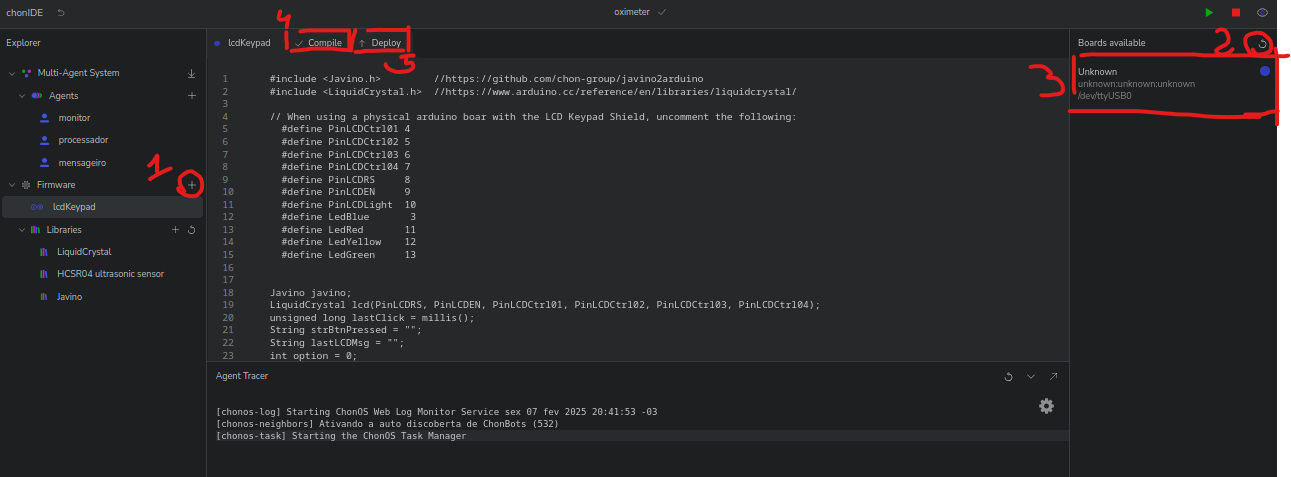
\includegraphics[width=0.8\textwidth]{assets/img/steps.png}
  \caption{Carrgando o Firmware}
  \label{fig:circuit}
\end{figure}

Feito isso, basta iniciar o projeto no botão de \textit{play} que as percepções começarão a ser elicitadas, sendo exibidas no console. Inicialmente, será exibido o valor de 98\% para o SPo2, nível considerado normal,  conforme figura a seguir.

\begin{figure}[H]
  \centering
  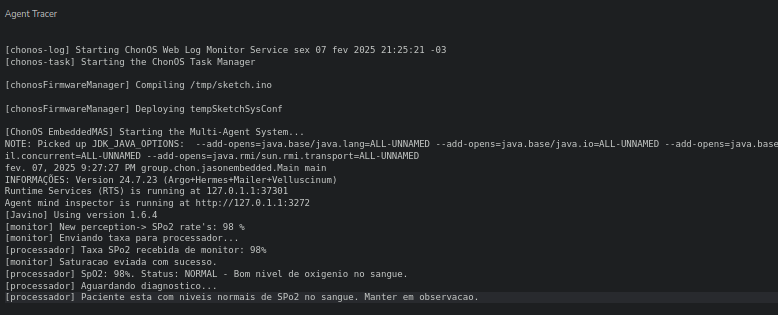
\includegraphics[width=0.8\textwidth]{assets/img/perceptions.png}
  \caption{Percepções Iniciais}
  \label{fig:circuit}
\end{figure}

Após isso, basta interagir com o teclado LCD para a regulação dos níveis de SPo2. Neste experimento, optou-se por demonstrar o comportamento do sistema para cada faixa risco. Então, foi feito o decremento dos níveis de SPo2 no teclado LCD, de forma a atingir tal patamar. O resultado dessa ação pode ser melhor observado na figura a seguir.

\begin{figure}[H]
  \centering
  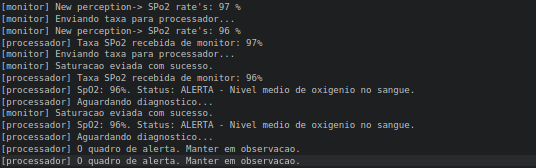
\includegraphics[width=0.8\textwidth]{assets/img/perception.alert.png}
  \caption{Percepção de Alerta}
  \label{fig:circuit}
\end{figure}

Reduzindo um pouco mais, para níveis abaixo de 92\%, é possível observar o cenário de caso crítico, conforme demonstrado na imagem abaixo. 

\begin{figure}[H]
  \centering
  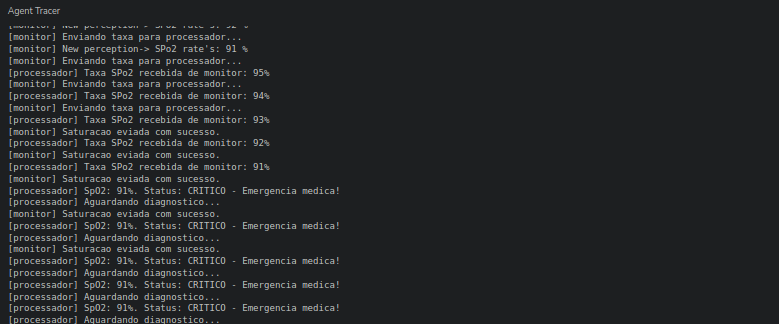
\includegraphics[width=0.8\textwidth]{assets/img/perception.emergency.png}
  \caption{Estado Crítico}
  \label{fig:circuit}
\end{figure}

Ao atingir esse patamar, nota-se a comunicação entre o agente \textbf{processador} e o \textbf{mensageiro}, uma vez que a condição de acionamento por status é atingida no primeiro agente. Com isso, a rede de apoio cadastrada no \textbf{mensageiro} é devidamente notificada, conforme image a seguir.

\begin{figure}[H]
  \centering
  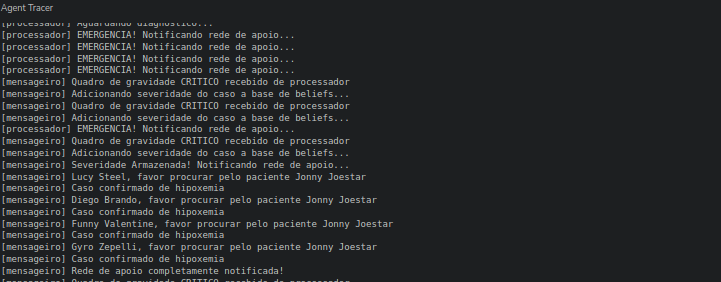
\includegraphics[width=0.8\textwidth]{assets/img/netwokcall.png}
  \caption{Contactando Rede}
  \label{fig:circuit}
\end{figure}

E com isso, o experimento é finalizado, contemplado todos os diagnósticos propostos no projeto e, quando necessário, notificando a rede.

% No caso deste projeto, foi usada uma variante do firmware \textbf{\textit{Arduino LCD Keypad Project}} \cite{ArgoAgent} \footnote{Este projeto está disponível gratuitamente em \href{https://github.com/chon-group/Argo/wiki/Arduino-LCD-Keypad-Project}{Github/chon-group}}. Ela sofreu modificação quanto às percepções programadas, que foram adaptadas para parâmetros biométricos, como SPo2 e BPM, usados neste projeto.

% % Snippet Chon
% \lstinputlisting[
%     style=c++,
%     caption={Parâmetros Biométricos}
%     ,
%     firstline=62,  
%     lastline=67
% ]{code/oximeterSketch.ino}

